The purpose of this thesis is to reduce the latency of graph access in cases
where the graph is stored on a distributed file system like AWS S3. To
put this work into context, we start by providing an overview of distributed
storage services and more details about the particular storage service that
will be used in this thesis. Then, we provide background on the idea of
separating compute and storage, the evolution of this idea, and its
applicability. After that, we describe the current literature on how others have
approached the idea of reducing access latency by using caching algorithms. We
end this section by comparing the contributions of this research with the
current state-of-the-art in the field of graph databases.

\section{Distributed storage services}\label{sec:distributedStorage}
The idea of accessing files via the network can be traced back to the early days
of the internet. However, the first widely used implementation of a networked
file system was developed by SUN Microsystems\cite{nfs1986}. Their implementation
is widely referred to as the networked file system (NFS). Their implementation
provided users with the ability to mount a file system present on a remote
machine. However, this system did not provide any distribution transparency, as
the users had to be aware of where and how each file was stored on remote
machines. 

\medskip
The first widely used implementation of a distributed file system is considered
to be the Hadoop Distributed File system (HDFS)\cite{shvachko2010hadoop}. This
implementation provided distribution transparency and consistency guarantees on
various operations on the files stored in HDFS. This implementation was inspired
by the Google File-system\cite{ghemawat2003google}, which was developed by Google
almost seven years before HDFS.

\medskip
Although systems like HDFS were widely used, distributed file systems like AWS
S3\cite{awsS3} provided an additional feature of being multi-tenant. In other
words, with file systems like AWS S3, a user could reap the benefits of a
distributed file system without having to manage or pay for an entire cluster.
The cost of managing, scaling, and maintaining the distributed cluster was
delegated to cloud providers like AWS. Now, users could pay for the amount of
data that they store, and the number of requests that they make to their data.
This has enabled the usage of such distributed file systems in applications like
video streaming, database storage\cite{snowflake}, web content 
delivery, and backup storage.

\begin{figure}[ht]
    \centering
    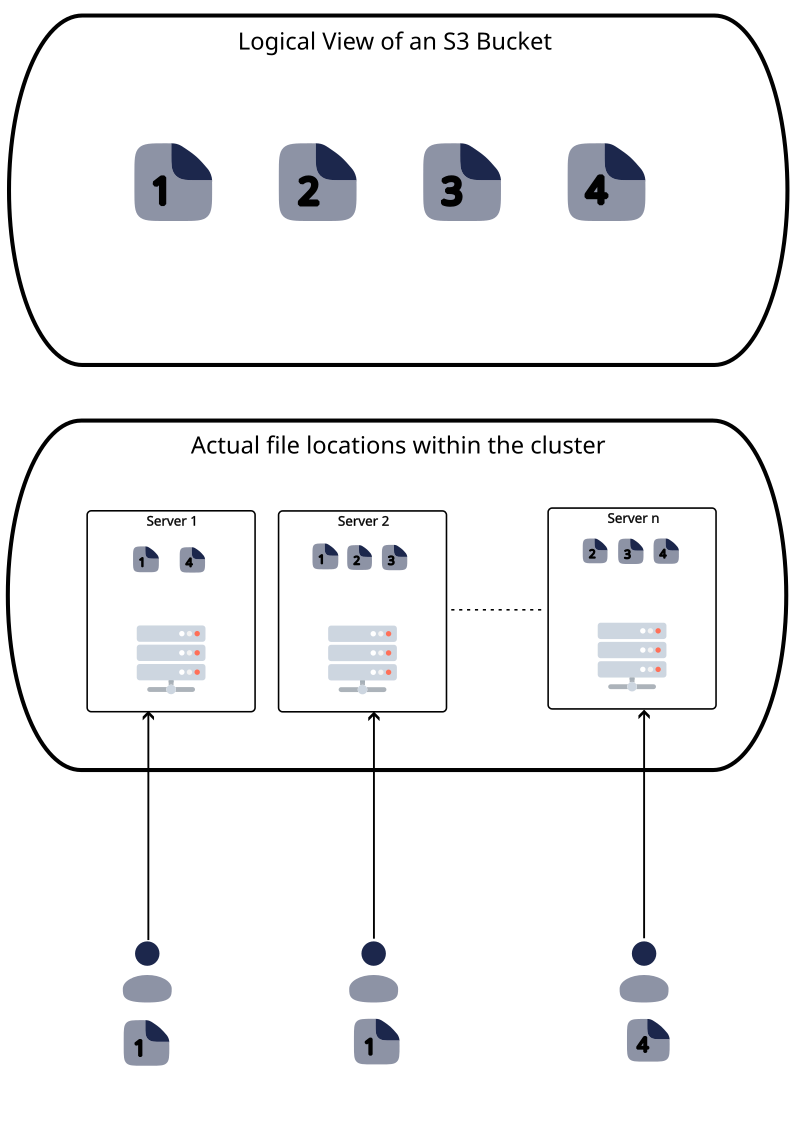
\includegraphics[width=0.65\textwidth]{figures/distributedCloudStorage.png}
    \caption{Distributed File Store}
    \label{fig:distFileStore}
\end{figure}

\medskip
The exact architecture of AWS S3 or any similar service provided by
competing cloud providers is not known precisely. However, we can glean some information
about S3 based on
how other distributed file systems were designed. We will explain some basic ideas
related to AWS S3 using Figure-\ref{fig:distFileStore}. Let us assume we need to
store four files in AWS S3. To do that, we first create a storage unit
called a `bucket', which is similar to a directory in a file system. After
uploading our files to this bucket, the files get replicated over the entire AWS S3 cluster in
that particular region. Figure-\ref{fig:distFileStore} assumes that this cluster
has a replication factor of two, and therefore, every file is stored on two
physical servers. Now, if users send requests to access these files, their
requests can be redirected to any one of the servers containing the desired file. For
example, if the first and the second user both want to access file number 1, their
requests can be served by two different servers since the same copy will be
saved on two different servers. For simplicity, the figure shows that users make
direct requests to the physical machines containing these files. However, in
reality, they all send requests to a single endpoint, and their requests are then
redirected to a server based on some load-balancing scheme. In later chapters,
we will use this abstract model of a distributed file system to argue about the
applicability of various techniques.

\medskip
Apart from the basic understanding of AWS S3 as it relates to a distributed
file system, we also want to draw the reader's attention to the following
characteristics of AWS S3 as mentioned in its documentation:
\begin{enumerate}
    \item \textbf{Throughput SLA}: At the time of writing this paper, AWS
        guarantees that S3 can handle at least 5500 requests per object stored
        in a bucket. Note that there is no restriction on the total number of
        objects that can be stored in a bucket.
    \item \textbf{Storage Classes}: S3 offers various storage classes that have
        different cost and performance characteristics. These storage classes
        determine how much you pay for storage and for making requests. In this
        thesis, we make use of the `S3 Standard' and `Express One Zone' storage
        classes.
    \item \textbf{Costs}: The cost of using AWS S3 depends on two factors: total
        storage and number of requests. The storage cost for `S3 Standard'
        storage class is \$0.023/GB and the cost of GET requests is
        \$0.0004/1k requests. However, the storage cost for the lower latency
        `Express One Zone' storage type is higher with \$0.16/GB, but the cost of making
        requests is lower at \$0.0002/1k requests. 
    \item \textbf{Artificial sub-directories}: Although AWS CLI and other tools
        provide the capability to upload and navigate a bucket like a directory,
        the underlying architecture only supports having files inside a
        bucket. Therefore, if you have a folder `f1' with two files `one' and
        `two', unlike a file system, the bucket would only contain two files:
        `f1/one' and `f1/two'. The name of the folder is
        prepended to the file names.
    \item \textbf{Hashing object names}: To decide which partitions an
        object is assigned to, S3 internally hashes the first few characters of
        the filename. Therefore, if we have object names whose first few
        characters are the same, they may all be assigned to a
        single partition, which may lead to lower performance. Although it is
        known that S3 automatically splits partitions in case of overload,
        there is some overhead and time delay in performing the split.
    \item \textbf{Consistency}: Despite being a distributed system, AWS S3
        provides a strong `Read-After-Write' consistency. This means that any
        updates to an object are immediately visible to all clients.
\end{enumerate}

\section{Separating compute and storage}\label{sec:serverlessArch}
One of the first proposed implementations of a database with separate compute and
storage can be traced back to 2008\cite{brantner2008building}, where Brantner et
al. proposed an architecture of a relational database that used AWS S3 as its
storage layer. The authors of this paper primarily focused on how to handle
updates under various consistency models when the data is stored in S3. This
idea was further developed over the years by AWS and culminated with the release
of AWS Aurora\cite{verbitski2017amazon}. Although Aurora separated compute and
storage, the write throughput was still limited because all write
traffic was directed to a single instance. The first database to support
multiple read and write instances on top of distributed data is considered to be
Snowflake\cite{dageville2016snowflake}. Their architecture was built upon the
storage layer of AWS S3. On top of this storage layer, users could create as many `virtual
warehouses' as they needed. Since then, various databases with independent
storage and compute planes like Neon\cite{neonPostgres} and AWS Aurora
Serverless\cite{auroraServerless} have been released.

\medskip
The term `Serverless databases' is often used for databases with separate
compute and storage; however, these two concepts are different. A `serverless
database' has a pay-as-you-go model where you pay for the amount of storage that
your databases use, and the compute resources that were used in a fixed amount
of time. In this model, the users simply have to define the minimum and maximum
compute resources that the database can use and the database scales according
to the load. Note that the definition of serverless database does not
necessitate separation between compute and storage, and there are indeed
databases like CockroachDB\cite{taft2020cockroachdb} which offer a serverless
model although the underlying architecture couples storage and compute together.
Therefore, although separating compute and storage may be amenable to a
serverless design, it is not a requirement for it. The term serverless,
therefore, defines a type of payment model, whereas having separate storage and
compute for a database is more of a system architecture choice. 

\medskip
A database that separates compute and storage offers better scalability,
elasticity, and modularity. When the compute and storage are
separated, both of them can be scaled independently. A heavily used service
that has a relatively low amount of data can scale the database's compute without
wasting any storage. On the other hand, a service that has a lot of data but
has a low query workload can scale the database's storage without wasting any
compute. Furthermore, this separation also provides more elasticity so that the
database can seamlessly scale up when the workload increases and can scale down
during low-traffic hours. Finally, separating storage and compute can lead to
more modularity since the storage layer and the compute layer can be upgraded
and changed based on the system's requirements. For example, if a cloud provider
launches a new instance type that is better suited for your workload, you can
switch to the newer instance type without being concerned about data migration.
These aforementioned characteristics make databases with separate compute and
storage attractive to a variety of use cases.

\medskip
Separating compute and storage in databases often comes at the cost of increased
latency. This latency is a result of the network communication between the
storage layer and compute layer that needs to take place to complete any
database operation. Although the throughput of networks has massively increased
in the past few years (AWS offers instances with up to 200 Gbps bandwidth), the
latency of network communication is limited by the speed of light. Therefore, a
database with a local SSD containing all the base data will always be faster
than a database whose storage needs to be accessed over a network. The actual
difference between performance depends on the physical distance between storage
and compute nodes. If the entire deployment is in a single data center, the
latency is around 500$\mu$s, which is still an order of magnitude higher than access latency
for an SSD\cite{jiang2021fusionraid}. This advantage becomes less pronounced in
distributed databases with coupled storage and compute since they may also require
some communication between instances to respond to user queries.
Although there are various caching and prefetching mechanisms to reduce latency
for databases with separate storage and compute, there remain cases where
coupling storage and compute yields lower latencies.


\section{Caching and Prefetching}\label{sec:cachingDistSys}
The concept of caching and prefetching in the case of graphs enables us to take
advantage of spatial and temporal locality to reduce the latency of future graph
accesses. The terms spatial and temporal locality come from literature on
processor caches. In the context of a processor cache, temporal locality refers
to the tendency of a memory location that is accessed now to be
accessed again soon. Similarly, spatial locality refers to the 
tendency of a memory location close to a recently accessed memory location to be
accessed in the near future. These concepts can be translated to graphs as
follows:
\begin{enumerate}
    \item \textbf{Spatial Locality} in case of graphs means that if a node is
        accessed, then it is likely that this node's neighbors will be accessed
        in the near future.
    \item \textbf{Temporal Locality} in case of graphs refers to the existence
        of central nodes according to some centrality metric. There are
        various centrality measures\cite{klein2010centrality}, which may help us 
        identify nodes that are central for a particular graph algorithm. The
        main idea is that there exist some nodes that have a higher probability
        of being accessed while running a particular algorithm on a graph.
\end{enumerate}
In this section, we will discuss some background research on caching and
prefetching, which would help us exploit  spatial and temporal locality to lower
the data access latency for graph traversals.

\medskip
Any caching scheme consists of two fundamental operations: admission of
data to the cache and eviction of data from the cache. There are various cache
eviction policies like Least Recently Used (LRU), Least Frequently Used (LFU)
that define what data to evict from the cache when it becomes
full. There also exist eviction policies that rely on metadata related to the
data to choose the data elements to evict. Such metadata might
include the size of the data element, time of last data access, and access latency
of the element in case of a cache miss. Apart from eviction, a cache also needs
an admission policy, which, in the case of most caches, is to add the data that
caused a cache miss. However, there do exist more sophisticated
admission algorithms like TinyLFU\cite{einziger2017tinylfu}, which make the
admission decision based on metadata related to a data object, which in the case of
TinyLFU is the access frequency of a data item. Storing metadata of an
object often increases memory consumption and maintenance overhead. These
admission and eviction policies determine the effectiveness of a cache algorithm
for a given use case.

\medskip
We will first consider schemes that do not require additional information about
the stored data, like size or access latency, in case of a cache miss. In
this case, LRU and LFU are two of the most commonly used algorithms. It has been
shown that if the access pattern follows Zipf's law\cite{zipf1929relative}, then
LFU outperforms LRU. However, if the access pattern has a high temporal locality,
then LRU can outperform LFU. Therefore, the choice between LRU and LFU depends
on the underlying access pattern of the data. This choice, however, does not
have to be binary as we can also have an LRFU cache\cite{lee2001lrfu}, which
provides us with a way to have an eviction policy that takes both recency and
frequency into account for eviction. This algorithm subsumes both LRU and LFU
because its functioning depends on a factor $\lambda$, which dictates the
weight that is given to recency versus frequency while evicting an item. As a
result, we can tune this parameter to have the cache behave like LRU or LFU.
Thus, with the LRFU cache, we can fine-tune our eviction policy when we do not
have additional information about the items.

\medskip
In the last paragraph, we talked about caching policies when we do not have any
additional information about the stored items; however, while processing
graphs, we do have some information about the graph topology when we access a
node's neighbors. This information can be useful if a node's neighbors are
likely to be accessed. This idea of graph-aware
caching algorithms was introduced by Aksu et al. in a paper where they
introduced a graph-aware caching policy named Clock-based graph-aware
caching (CBGA)\cite{aksu2015graph}. Although the algorithm contains many 
important contributions, the
main idea of this algorithm is to expect that a node's neighbors will be
accessed if a node is accessed. This idea helped their algorithm outperform all
other competing cache algorithms, which did not exploit the structure of the
graph. Their idea was further extended by Bok et al.\cite{bok2020memory}, where
they added a used-cache in addition to a prefetcher cache for speeding up
sub-graph lookups. This idea helped them outperform CBGA for the task of sub-graph
matching where they achieved a hit ratio of between 50\% and 65\%. 
These contributions highlight the potential for graph-aware caching to
reduce the latency of graph access.

\section{Comparison with State-of-the-Art}\label{sec:cmpSOTA}
In the field of graph databases, there are two types of databases based on how
they store the underlying graph data: native graph databases and non-native graph
databases. Native graph databases (like Neo4j\cite{neo4j}) use data structures that are 
optimized for
graph traversals and thus, usually deliver better performance for graph
navigation operations. Non-native graph databases (like Amazon Neptune\cite{neptune}) rely 
on storage mechanisms of
relational databases, key-value stores, or document stores to store the
underlying graph. In this paper, we propose an architecture that leverages
distributed storage services to store graphs in a native graph data structure. 


\smallskip
This architecture is a unique contribution because most native graph databases 
couple storage and compute together. Graph databases like Neo4j and
Memgraph\cite{memgraph} require all the
data to be present on a single machine. Although Neo4j supports sharding of
graph data, the onus of doing so is primarily put on the user. There are some
closed-source databases like Tigergraph\cite{tigergraph} that support automatic sharding, 
but the storage and compute are tied together. In this landscape of graph 
databases, we aim to explore the
viability of a graph storage architecture that leverages distributed storage
systems. In this architecture, all the graph data would be present on the
distributed file system, and queries on this data would be served by stateless
compute instances. This separation would provide bottomless storage and the
ability to scale up or scale down compute easily. This ability to deliver
practically infinite storage and compute elasticity is a feature missing from
most native graph databases.
